%%%%%%%%%%%%%%%%%%%%%%%%%%%%%%%%%%%%%%%%%
% Beamer Presentation
% LaTeX Template
% Version 2.0 (March 8, 2022)
%
% This template originates from:
% https://www.LaTeXTemplates.com
%
% Author:
% Vel (vel@latextemplates.com)
%
% License:
% CC BY-NC-SA 4.0 (https://creativecommons.org/licenses/by-nc-sa/4.0/)
%
%%%%%%%%%%%%%%%%%%%%%%%%%%%%%%%%%%%%%%%%%

%----------------------------------------------------------------------------------------
%	PACKAGES AND OTHER DOCUMENT CONFIGURATIONS
%----------------------------------------------------------------------------------------

\documentclass[
	11pt, % Set the default font size, options include: 8pt, 9pt, 10pt, 11pt, 12pt, 14pt, 17pt, 20pt
	%t, % Uncomment to vertically align all slide content to the top of the slide, rather than the default centered
	aspectratio=169, % Uncomment to set the aspect ratio to a 16:9 ratio which matches the aspect ratio of 1080p and 4K screens and projectors
]{beamer}

\graphicspath{{figures/}{./}} % Specifies where to look for included images (trailing slash required)

\usepackage{booktabs} % Allows the use of \toprule, \midrule and \bottomrule for better rules in tables
\usepackage{subcaption}
%----------------------------------------------------------------------------------------
%	SELECT LAYOUT THEME
%----------------------------------------------------------------------------------------

% Beamer comes with a number of default layout themes which change the colors and layouts of slides. Below is a list of all themes available, uncomment each in turn to see what they look like.

% \usetheme{default}
%\usetheme{AnnArbor}
%\usetheme{Antibes}
% \usetheme{Bergen}
%\usetheme{Berkeley}
%\usetheme{Berlin}
%\usetheme{Boadilla}
%\usetheme{CambridgeUS}
%\usetheme{Copenhagen}
%\usetheme{Darmstadt}
% \usetheme{Dresden}
%\usetheme{Frankfurt}
%\usetheme{Goettingen}
%\usetheme{Hannover}
%\usetheme{Ilmenau}
%\usetheme{JuanLesPins}
%\usetheme{Luebeck}
\usetheme{Madrid}
%\usetheme{Malmoe}
%\usetheme{Marburg}
%\usetheme{Montpellier}
%\usetheme{PaloAlto}
%\usetheme{Pittsburgh}
%\usetheme{Rochester}
%\usetheme{Singapore}
%\usetheme{Szeged}
%\usetheme{Warsaw}

%----------------------------------------------------------------------------------------
%	SELECT COLOR THEME
%----------------------------------------------------------------------------------------

% Beamer comes with a number of color themes that can be applied to any layout theme to change its colors. Uncomment each of these in turn to see how they change the colors of your selected layout theme.

%\usecolortheme{albatross}
%\usecolortheme{beaver}
%\usecolortheme{beetle}
%\usecolortheme{crane}
%\usecolortheme{dolphin}
%\usecolortheme{dove}
%\usecolortheme{fly}
%\usecolortheme{lily}
%\usecolortheme{monarca}
%\usecolortheme{seagull}
%\usecolortheme{seahorse}
%\usecolortheme{spruce}
%\usecolortheme{whale}
%\usecolortheme{wolverine}

%----------------------------------------------------------------------------------------
%	SELECT FONT THEME & FONTS
%----------------------------------------------------------------------------------------

% Beamer comes with several font themes to easily change the fonts used in various parts of the presentation. Review the comments beside each one to decide if you would like to use it. Note that additional options can be specified for several of these font themes, consult the beamer documentation for more information.

\usefonttheme{default} % Typeset using the default sans serif font
%\usefonttheme{serif} % Typeset using the default serif font (make sure a sans font isn't being set as the default font if you use this option!)
%\usefonttheme{structurebold} % Typeset important structure text (titles, headlines, footlines, sidebar, etc) in bold
%\usefonttheme{structureitalicserif} % Typeset important structure text (titles, headlines, footlines, sidebar, etc) in italic serif
%\usefonttheme{structuresmallcapsserif} % Typeset important structure text (titles, headlines, footlines, sidebar, etc) in small caps serif

%------------------------------------------------

%\usepackage{mathptmx} % Use the Times font for serif text
\usepackage{palatino} % Use the Palatino font for serif text

%\usepackage{helvet} % Use the Helvetica font for sans serif text
\usepackage[default]{opensans} % Use the Open Sans font for sans serif text
%\usepackage[default]{FiraSans} % Use the Fira Sans font for sans serif text
%\usepackage[default]{lato} % Use the Lato font for sans serif text
% bars for matrices
\newcommand*{\vertbar}{\rule[-1ex]{0.5pt}{2.5ex}}
\newcommand*{\horzbar}{\rule[.5ex]{2.5ex}{0.5pt}}

% gilles castel figures
\usepackage{import}
\usepackage{pdfpages}
\usepackage{transparent}
\usepackage{xcolor}
\newcommand{\incfig}[2][1]{%
    \def\svgwidth{#1\columnwidth}
    \import{./figures/}{#2.pdf_tex}
}
\pdfsuppresswarningpagegroup=1
%----------------------------------------------------------------------------------------
%	SELECT INNER THEME
%----------------------------------------------------------------------------------------

% Inner themes change the styling of internal slide elements, for example: bullet points, blocks, bibliography entries, title pages, theorems, etc. Uncomment each theme in turn to see what changes it makes to your presentation.

%\useinnertheme{default}
\useinnertheme{circles}
%\useinnertheme{rectangles}
%\useinnertheme{rounded}
%\useinnertheme{inmargin}

%----------------------------------------------------------------------------------------
%	SELECT OUTER THEME
%----------------------------------------------------------------------------------------

% Outer themes change the overall layout of slides, such as: header and footer lines, sidebars and slide titles. Uncomment each theme in turn to see what changes it makes to your presentation.

%\useoutertheme{default}
%\useoutertheme{infolines}
%\useoutertheme{miniframes}
%\useoutertheme{smoothbars}
%\useoutertheme{sidebar}
%\useoutertheme{split}
%\useoutertheme{shadow}
%\useoutertheme{tree}
%\useoutertheme{smoothtree}

%\setbeamertemplate{footline} % Uncomment this line to remove the footer line in all slides
%\setbeamertemplate{footline}[page number] % Uncomment this line to replace the footer line in all slides with a simple slide count

%\setbeamertemplate{navigation symbols}{} % Uncomment this line to remove the navigation symbols from the bottom of all slides

%----------------------------------------------------------------------------------------
%	PRESENTATION INFORMATION
%----------------------------------------------------------------------------------------

\title[3D Metric Fields]{3D Metric Fields} % The short title in the optional parameter appears at the bottom of every slide, the full title in the main parameter is only on the title page

\subtitle{Optimizing Frame Fields in a new Metric} % Presentation subtitle, remove this command if a subtitle isn't required

\author[Florin Achermann]{Florin Achermann} % Presenter name(s), the optional parameter can contain a shortened version to appear on the bottom of every slide, while the main parameter will appear on the title slide

\institute[Unibe]{University of Berne } % Your institution, the optional parameter can be used for the institution shorthand and will appear on the bottom of every slide after author names, while the required parameter is used on the title slide and can include your email address or additional information on separate lines

\date[\today]{Bachelor thesis \\ \today} % Presentation date or conference/meeting name, the optional parameter can contain a shortened version to appear on the bottom of every slide, while the required parameter value is output to the title slide

%----------------------------------------------------------------------------------------

\begin{document}

%----------------------------------------------------------------------------------------
%	TITLE SLIDE
%----------------------------------------------------------------------------------------

\begin{frame}
	\titlepage % Output the title slide, automatically created using the text entered in the PRESENTATION INFORMATION block above
\end{frame}

%----------------------------------------------------------------------------------------
%	TABLE OF CONTENTS SLIDE
%----------------------------------------------------------------------------------------

% The table of contents outputs the sections and subsections that appear in your presentation, specified with the standard \section and \subsection commands. You may either display all sections and subsections on one slide with \tableofcontents, or display each section at a time on subsequent slides with \tableofcontents[pausesections]. The latter is useful if you want to step through each section and mention what you will discuss.

\begin{frame}
	\frametitle{Presentation Overview} % Slide title, remove this command for no title
	
	\tableofcontents % Output the table of contents (all sections on one slide)
	%\tableofcontents[pausesections] % Output the table of contents (break sections up across separate slides)
\end{frame}

%----------------------------------------------------------------------------------------
%	PRESENTATION BODY SLIDES
%----------------------------------------------------------------------------------------

\section{Problem Statement} % Sections are added in order to organize your presentation into discrete blocks, all sections and subsections are automatically output to the table of contents as an overview of the talk but NOT output in the presentation as separate slides

%------------------------------------------------

\subsection{Hexahedral Meshing}

\begin{frame}
	\frametitle{Representation of geometry}
    Geometry needs to be represented in computers for applications
    
    \begin{figure}
        \begin{subfigure}{0.45\textwidth}
            \centering
            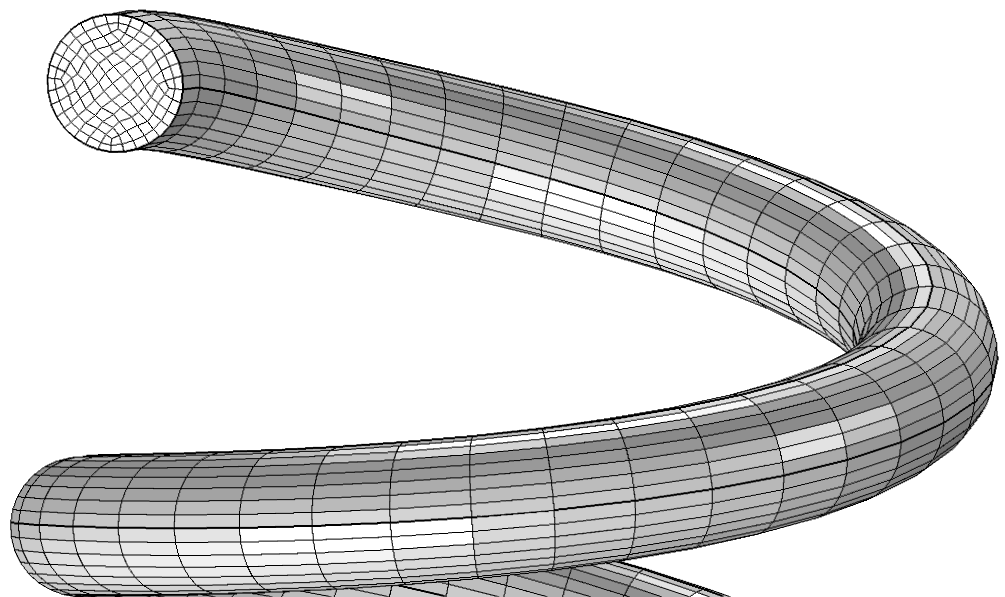
\includegraphics[width=\linewidth]{spiral.png}
            \caption{Hexahedral mesh of spring \textcopyright COMSOL}
            \label{fig:sub1}
        \end{subfigure}%
        \begin{subfigure}{0.45\textwidth}
            \centering
            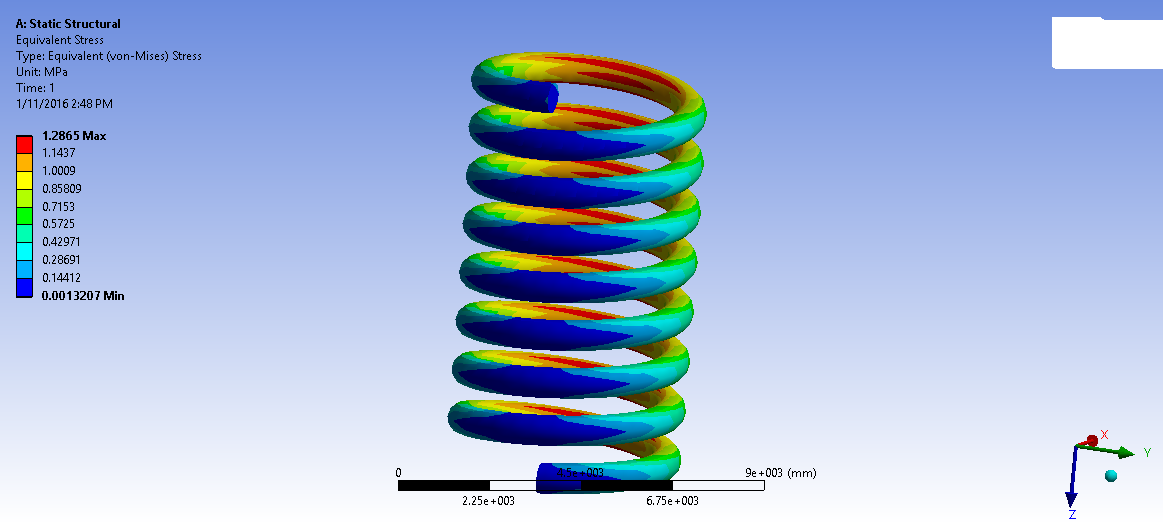
\includegraphics[width=\linewidth]{spring.png}
            \caption{Stress simulation on spring \textcopyright ANSYS}
            \label{fig:sub2}
        \end{subfigure}%
	\end{figure}
    Meshes out of hexahedral elements are prefered in practice
\end{frame}

%------------------------------------------------

\subsection{Integer-Grid Maps}
\begin{frame}
	\frametitle{Integer-Grid Maps}
	% \framesubtitle{Bullet Points and Numbered Lists} % Optional subtitle
	Key Idea: \\
	Search for map $\phi : \mathcal{M} \subset \mathbb{R}^3 \to \mathbb{R}^3$
	which maps the object to a 3D grid

	\begin{figure}
		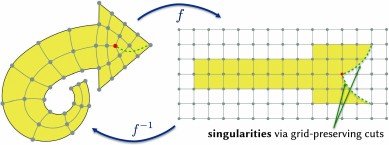
\includegraphics[width=0.5\linewidth]{integer-grid-rough.png}
		\caption{Integer-Grid map \cite{survey}}
	\end{figure}
	Direct search is infeasible $\rightarrow$ hard mixed-integer non-convex optimization problem	
\end{frame}
% \begin{frame}
	% \frametitle{Blocks of Highlighted Text}
	
	% \begin{block}{Block Title}
	% 	Lorem ipsum dolor sit amet, consectetur adipiscing elit. Integer lectus nisl, ultricies in feugiat rutrum, porttitor sit amet augue.
	% \end{block}
	
	% \begin{exampleblock}{Example Block Title}
	% 	Aliquam ut tortor mauris. Sed volutpat ante purus, quis accumsan.
	% \end{exampleblock}
	
	% \begin{alertblock}{Alert Block Title}
	% 	Pellentesque sed tellus purus. Class aptent taciti sociosqu ad litora torquent per conubia nostra, per inceptos himenaeos.
	% \end{alertblock}
	
	% \begin{block}{} % Block without title
	% 	Suspendisse tincidunt sagittis gravida. Curabitur condimentum, enim sed venenatis rutrum, ipsum neque consectetur orci.
	% \end{block}
% \end{frame}

%------------------------------------------------

\subsection{Frame Fields}
\begin{frame}
	\frametitle{Search for Integer-Grid Maps}
	We want:
	$$\phi : \mathcal{M} \to \mathbb{R}^3$$
	Idea: Take the Jacobian
	$$\nabla \phi : \mathcal{M} \to \mathbb{R}^{3\times3}$$
	and search for an approximation $F \approx \nabla \phi$. We call $F : \mathcal{M} \to \mathbb{R}^{3\times3}$ a \alert{frame field}.
	A \alert{frame} locally represents the deformed edges of a cube.
\end{frame}

\begin{frame}
	\frametitle{Frame Fields}
	\begin{columns}[c] % The "c" option specifies centered vertical alignment while the "t" option is used for top vertical alignment
	
		\begin{column}{0.6\textwidth} % Left column width
			Think of $F$ as three vector fields $F_i : \mathbb{R}^3 \to \mathbb{R}^3$
			$$F=\begin{pmatrix}
				\vertbar & \vertbar & \vertbar \\
				F_1 & F_2 & F_3 \\
				\vertbar & \vertbar & \vertbar
			\end{pmatrix}$$
			Goals for our frame field:
			\begin{itemize}
				\item Smoothness
				\item Boundary Alignment: One column should match with surface normal
			\end{itemize}
			Why?
		\end{column}
		\begin{column}{0.35\textwidth} % Right column width
			\begin{figure}
				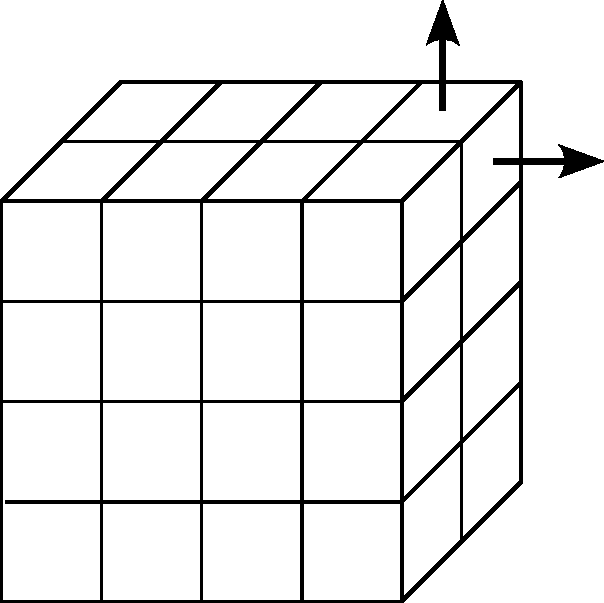
\includegraphics[width=\linewidth]{cube.pdf}
			\end{figure}
		\end{column}
	\end{columns}
\end{frame}

\begin{frame}
	\frametitle{Frame Fields}
	\begin{figure}
		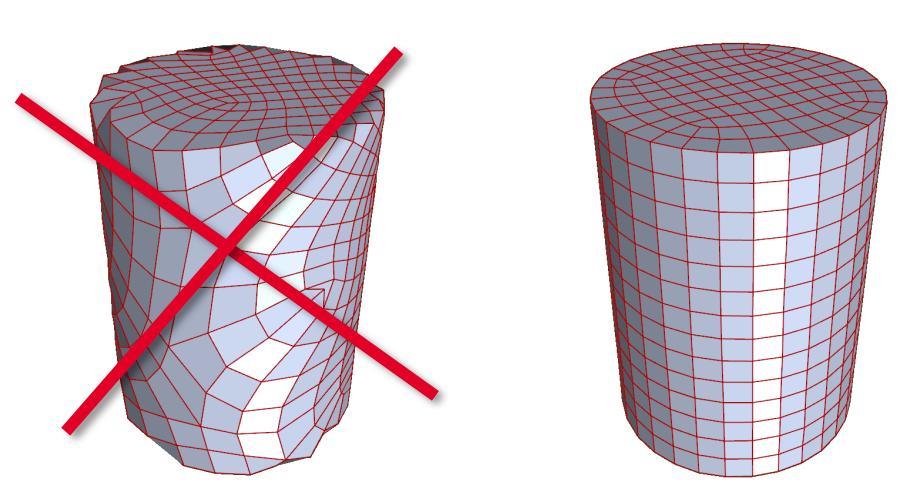
\includegraphics[width=0.7\linewidth]{requirements.png}
		\caption{Left: Missing Boundary Alignment, not smooth. Right: Smooth + Boundary Aligned \textcopyright CGG Bern, David Bommes}
	\end{figure}
\end{frame}

\begin{frame}
	\frametitle{Optimization Approach}
	\begin{itemize}
		\item Goal: Smooth Frame Field + Boundary Aligned
		\item How to measure smoothness? 
	\end{itemize}

	Dirichlet Energy
	\begin{equation}
		E(F) = \int_\mathcal{M} ||\nabla F||^2
	\end{equation}
\end{frame}

%------------------------------------------------

\section{Frame Field Control}

\subsection{Metric Fields}

\begin{frame}
	\frametitle{Controlling frames}
	\begin{columns}[c] % The "c" option specifies centered vertical alignment while the "t" option is used for top vertical alignment
	
		\begin{column}{0.5\textwidth} % Left column width
			\begin{itemize}
				\item For orthonormal frame field $F^TF = \mathrm{Id}$, extracted elements are unit cubes
				\item Add metric field $g$ for control of frames
				\item $g$-orthonormality $F^TgF = \mathrm{Id}$
			\end{itemize}
		\end{column}
		\begin{column}{0.45\textwidth} % Right column width
			\begin{figure}
				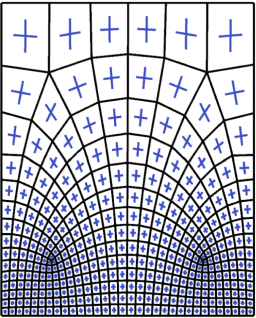
\includegraphics[width=0.6\linewidth]{factorization.png}
				\caption{Under new metric $g$, lengths at the top are the same lengths as at the bottom \cite{fang}}
			\end{figure}
		\end{column}
	\end{columns}
\end{frame}

% \begin{frame}
% 	\frametitle{Table}
% 	\framesubtitle{Subtitle} % Optional subtitle
	
% 	\begin{table}
% 		\begin{tabular}{l l l}
% 			\toprule
% 			\textbf{Treatments} & \textbf{Response 1} & \textbf{Response 2}\\
% 			\midrule
% 			Treatment 1 & 0.0003262 & 0.562 \\
% 			Treatment 2 & 0.0015681 & 0.910 \\
% 			Treatment 3 & 0.0009271 & 0.296 \\
% 			\bottomrule
% 		\end{tabular}
% 		\caption{Table caption}
% 	\end{table}
% \end{frame}

%------------------------------------------------

\subsection{Measuring Smoothness in new Metric}

\begin{frame}
	\frametitle{Space deformation}
	\begin{columns}[c] % The "c" option specifies centered vertical alignment while the "t" option is used for top vertical alignment
	
		\begin{column}{0.5\textwidth} % Left column width
			\begin{itemize}
				\item Metric $g$ measures deformation of space
				\item Cannot use euclidean smoothness measure
				\item $g$ defines infinitesimal rotation $\omega$
			\end{itemize}
		\end{column}
		\begin{column}{0.45\textwidth} % Right column width
			\begin{figure}
				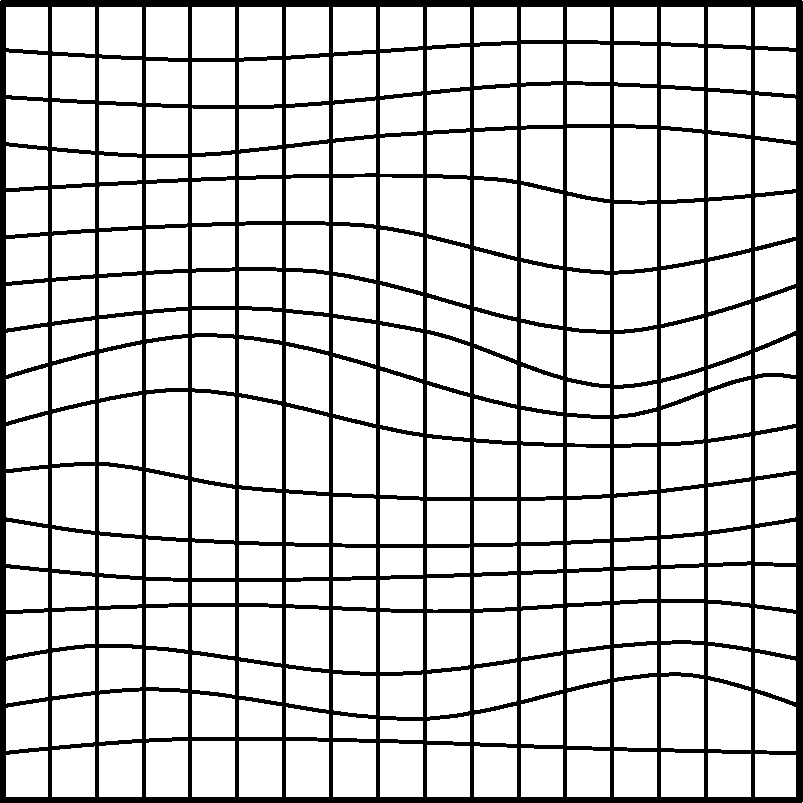
\includegraphics[width=0.8\linewidth]{lattice-grid.pdf}
				\caption{Metric $g$ deforms the space, ``straight'' in $g$ is not straight in euclidean metric}
			\end{figure}
		\end{column}
	\end{columns}
\end{frame}

\begin{frame}
	\frametitle{Measuring Smoothness in new Metric}
	\begin{figure}[htb]
		\centering
		\def\svgwidth{0.5\linewidth}
		\input{figures/rotation.pdf_tex}
		\caption{Under the metric induced by $\phi$, the frame at $q$ is parallel to $p$.
		To compare them, we need to recover how $p$ is rotated under $\omega$.}
		\label{fig:rotation}
	\end{figure}
\end{frame}

%------------------------------------------------

\section{Discretization}

\begin{frame}
	\frametitle{Discretizing metric field}
	\begin{columns}[c] % The "c" option specifies centered vertical alignment while the "t" option is used for top vertical alignment
	
		\begin{column}{0.65\textwidth} % Left column width
			\begin{figure}[htb]
				\centering
				\def\svgwidth{0.6\linewidth}
				\input{figures/discretization.pdf_tex}
				\label{fig:discretization}
			\end{figure}
			We cover the object with a tetrahedral mesh and store
			the metrics at the vertices. Within the tet, we linearly interpolate with barycentric coordinates.
		\end{column}
		\begin{column}{0.35\textwidth} % Right column width
			\begin{figure}[htb]
				\centering
				\def\svgwidth{\linewidth}
				\input{figures/tet.pdf_tex}
				% \caption{}
				\label{fig:tet}
			\end{figure}
			$g=\alpha g_1 + \beta g_2 + \gamma + g_3 + \delta g_4$ with $\alpha+\beta+\gamma+\delta=1$
			and $\alpha,\beta,\gamma,\delta \ge 0$
		\end{column}
	\end{columns}
\end{frame}

%------------------------------------------------

\begin{frame}
	\frametitle{Walking on a triangulation}
	\begin{itemize}
		\item Problem: When integrating from $q$ to $p$, need
		to use appropriate metric field.
		\item Need to find all tets that the line segment from $q$ to $p$ lies in to
		do integration in correct field
		\begin{figure}[htb]
			\centering
			\def\svgwidth{0.9\linewidth}
			\input{figures/problem.pdf_tex}
			% \caption{}
			\label{fig:problem}
		\end{figure}
	\end{itemize}
	
\end{frame}

\begin{frame}
	\frametitle{Walking on a triangulation}
	\begin{figure}[htb]
		\centering
		\def\svgwidth{0.8\linewidth}
		\input{figures/illustration.pdf_tex}
		% \caption{}
		\label{fig:walking}
	\end{figure}
\end{frame}

\begin{frame}
	\frametitle{Putting all together}
	\begin{enumerate}
		\item Store metric field at vertices
		\item Minimize discretized Dirichlet energy with minimizer
		\begin{equation}
			E(F)=\int_{\mathcal{M}}||\nabla F||^2 \longrightarrow E(F)= \sum_{i,j} ||F_i-F_j||^2
		\end{equation}
		\item modify with rotation coefficient to align in new metric
		\begin{equation}
			E(F)= \sum_{q,p} ||[R_{qp}]F_q-F_p||^2
		\end{equation}
	\end{enumerate}
\end{frame}

\begin{frame}
	\frametitle{Experiments}
	\begin{columns}[c] % The "c" option specifies centered vertical alignment while the "t" option is used for top vertical alignment
	
		\begin{column}{0.25\textwidth} % Left column width
			$$g=\begin{pmatrix}
				1 & 0 & 0 \\ 0 & 1 & 0 \\ 0 & 0 & 1
			\end{pmatrix}$$
		\end{column}
		\begin{column}{0.7\textwidth} % Right column width
			\begin{figure}
				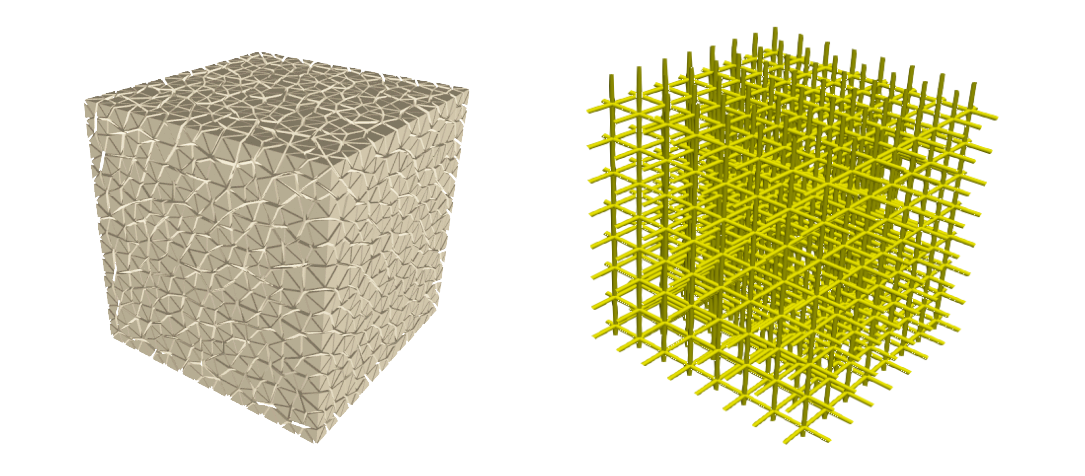
\includegraphics[width=\linewidth]{image1.png}
				\caption{Constant metric everywhere, constant frame field}
			\end{figure}
		\end{column}
	\end{columns}
\end{frame}
\begin{frame}
	\frametitle{Experiments}	
	\begin{equation}
		g(z) = \begin{cases}
			\mathrm{diag}(1,1,1) &0 < z < 1/3 \\
			\mathrm{diag}(27z-8,1,27z-8) &1/3 < z < 2/3 \\
			\mathrm{diag}(10,1,10) &2/3 < z < 1 \\
	\end{cases}\end{equation}\label{eq:metric}
	\begin{figure}
		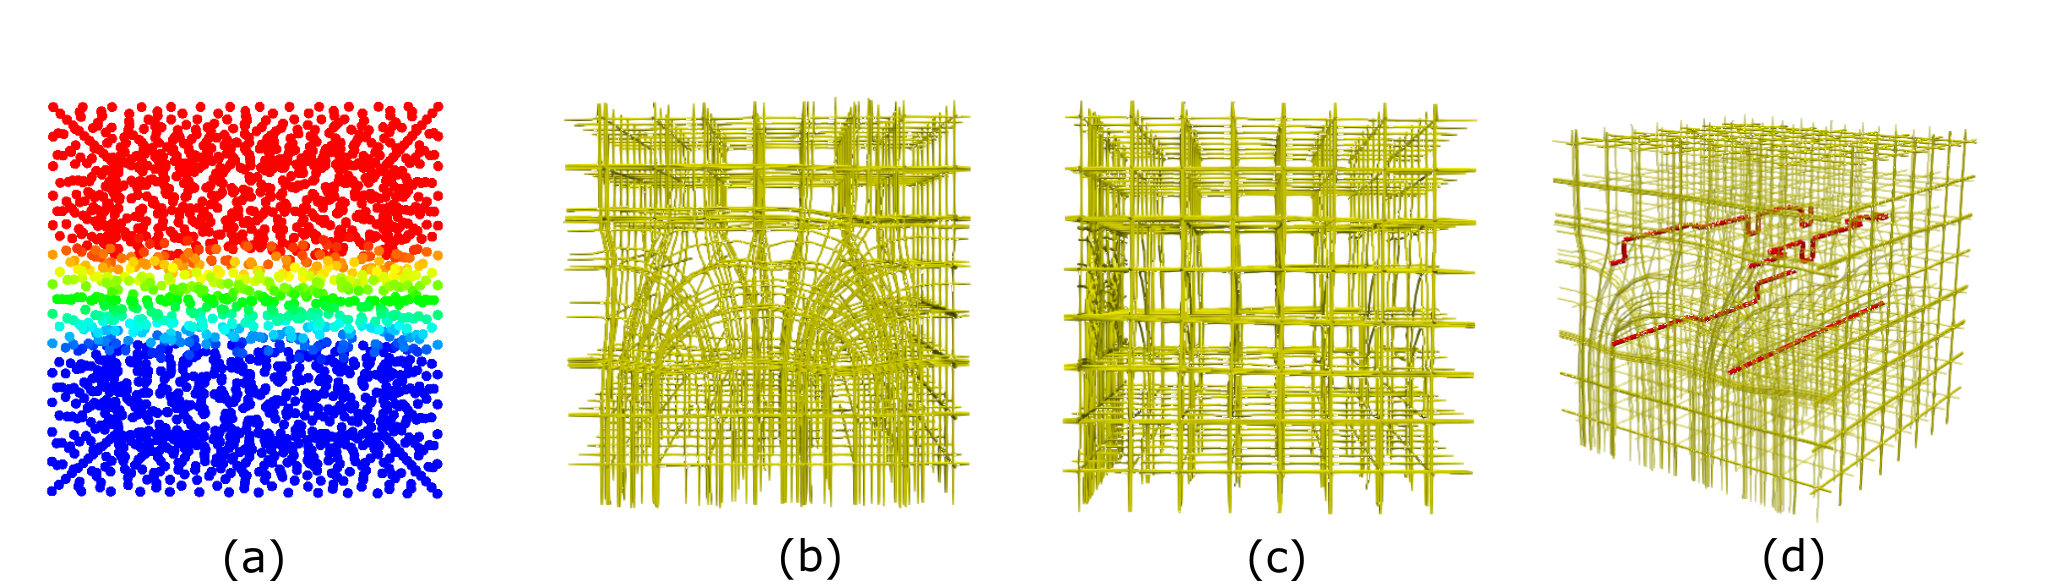
\includegraphics[width=0.9\linewidth]{image2.png}
		\caption{Constant-linear-constant metric}
	\end{figure}
\end{frame}
\frame

%------------------------------------------------

\begin{frame} % Use [allowframebreaks] to allow automatic splitting across slides if the content is too long
	\frametitle{References}
	
	\begin{thebibliography}{99} % Beamer does not support BibTeX so references must be inserted manually as below, you may need to use multiple columns and/or reduce the font size further if you have many references
		\footnotesize % Reduce the font size in the bibliography
		
		\bibitem[Pietroni et al., 2022]{survey}
			Pietroni et al. (2022)
			\newblock Hex-Mesh Generation and Processing: A Survey
			\newblock \emph{ACM Transaction on Graphics}
			
		\bibitem[Fang et al., 2023]{fang}
			Fang et al. (2023)
			\newblock Metric-Driven 3D Frame Field Generation
			\newblock \emph{IEEE Transactions on Visualization and Computer Graphics}.
	\end{thebibliography}
\end{frame}

%----------------------------------------------------------------------------------------
%	CLOSING SLIDE
%----------------------------------------------------------------------------------------

\begin{frame}[plain] % The optional argument 'plain' hides the headline and footline
	\begin{center}
		{\Huge The End}
		
		\bigskip\bigskip % Vertical whitespace
		
		{\LARGE Questions? Comments?}
	\end{center}
\end{frame}

%----------------------------------------------------------------------------------------

\end{document} 